\subsection{Structure and mechanics}

\paragraph{}The design and operation of a CubeSat is a complex process that must be completed keeping in mind the different subsystems as well as the role they will play during the lifetime of the mission. And since these systems will operate in space, they have to be prepared and certified to withstand extreme temperature and radiation conditions.

\paragraph{}The satellite used by Astrea must have high compatibility between all the systems to avoid potential problems and has to be tested (either all the systems together or one by one) and their correct functioning has to be ensured. Given that the lifetime of the mission should be greater than four years, the critical systems such as the solar arrays, batteries and antennas should be fully operational until the end of the mission.

\subsubsection{Structure}

\paragraph{}The mission of the structure is to sustain and protect all the electronic devices carried by the satellite in order to fulfill the mission requirements. In order to ensure that all the electronic and mechanic systems can be mounted upon the structure, a high compatibility between these systems is required. Given that the configuration of the current CubeSat is not as common as other configurations of actual commercial or operational CubeSats, it is a really important point that the structure is highly flexible regarding the arrangement of the subsystems.

\paragraph{}The structure chosen is manufactured by \textbf{Innovative Solutions In Space (ISIS)}. Among its features it is worth mentioning that it can withstand the high range of temperature it will face in the space (from -40ºC to 80ºC) and it is highly compatible; almost every physical system  used can be placed within the structure or on its faces (such as the antennas or the deployable solar arrays). Finally, the mass of the structure is relatively low, and given that the mass of the other subsystems is sometimes a drawback, it is plus point.
%
%\begin{figure}[h!]
%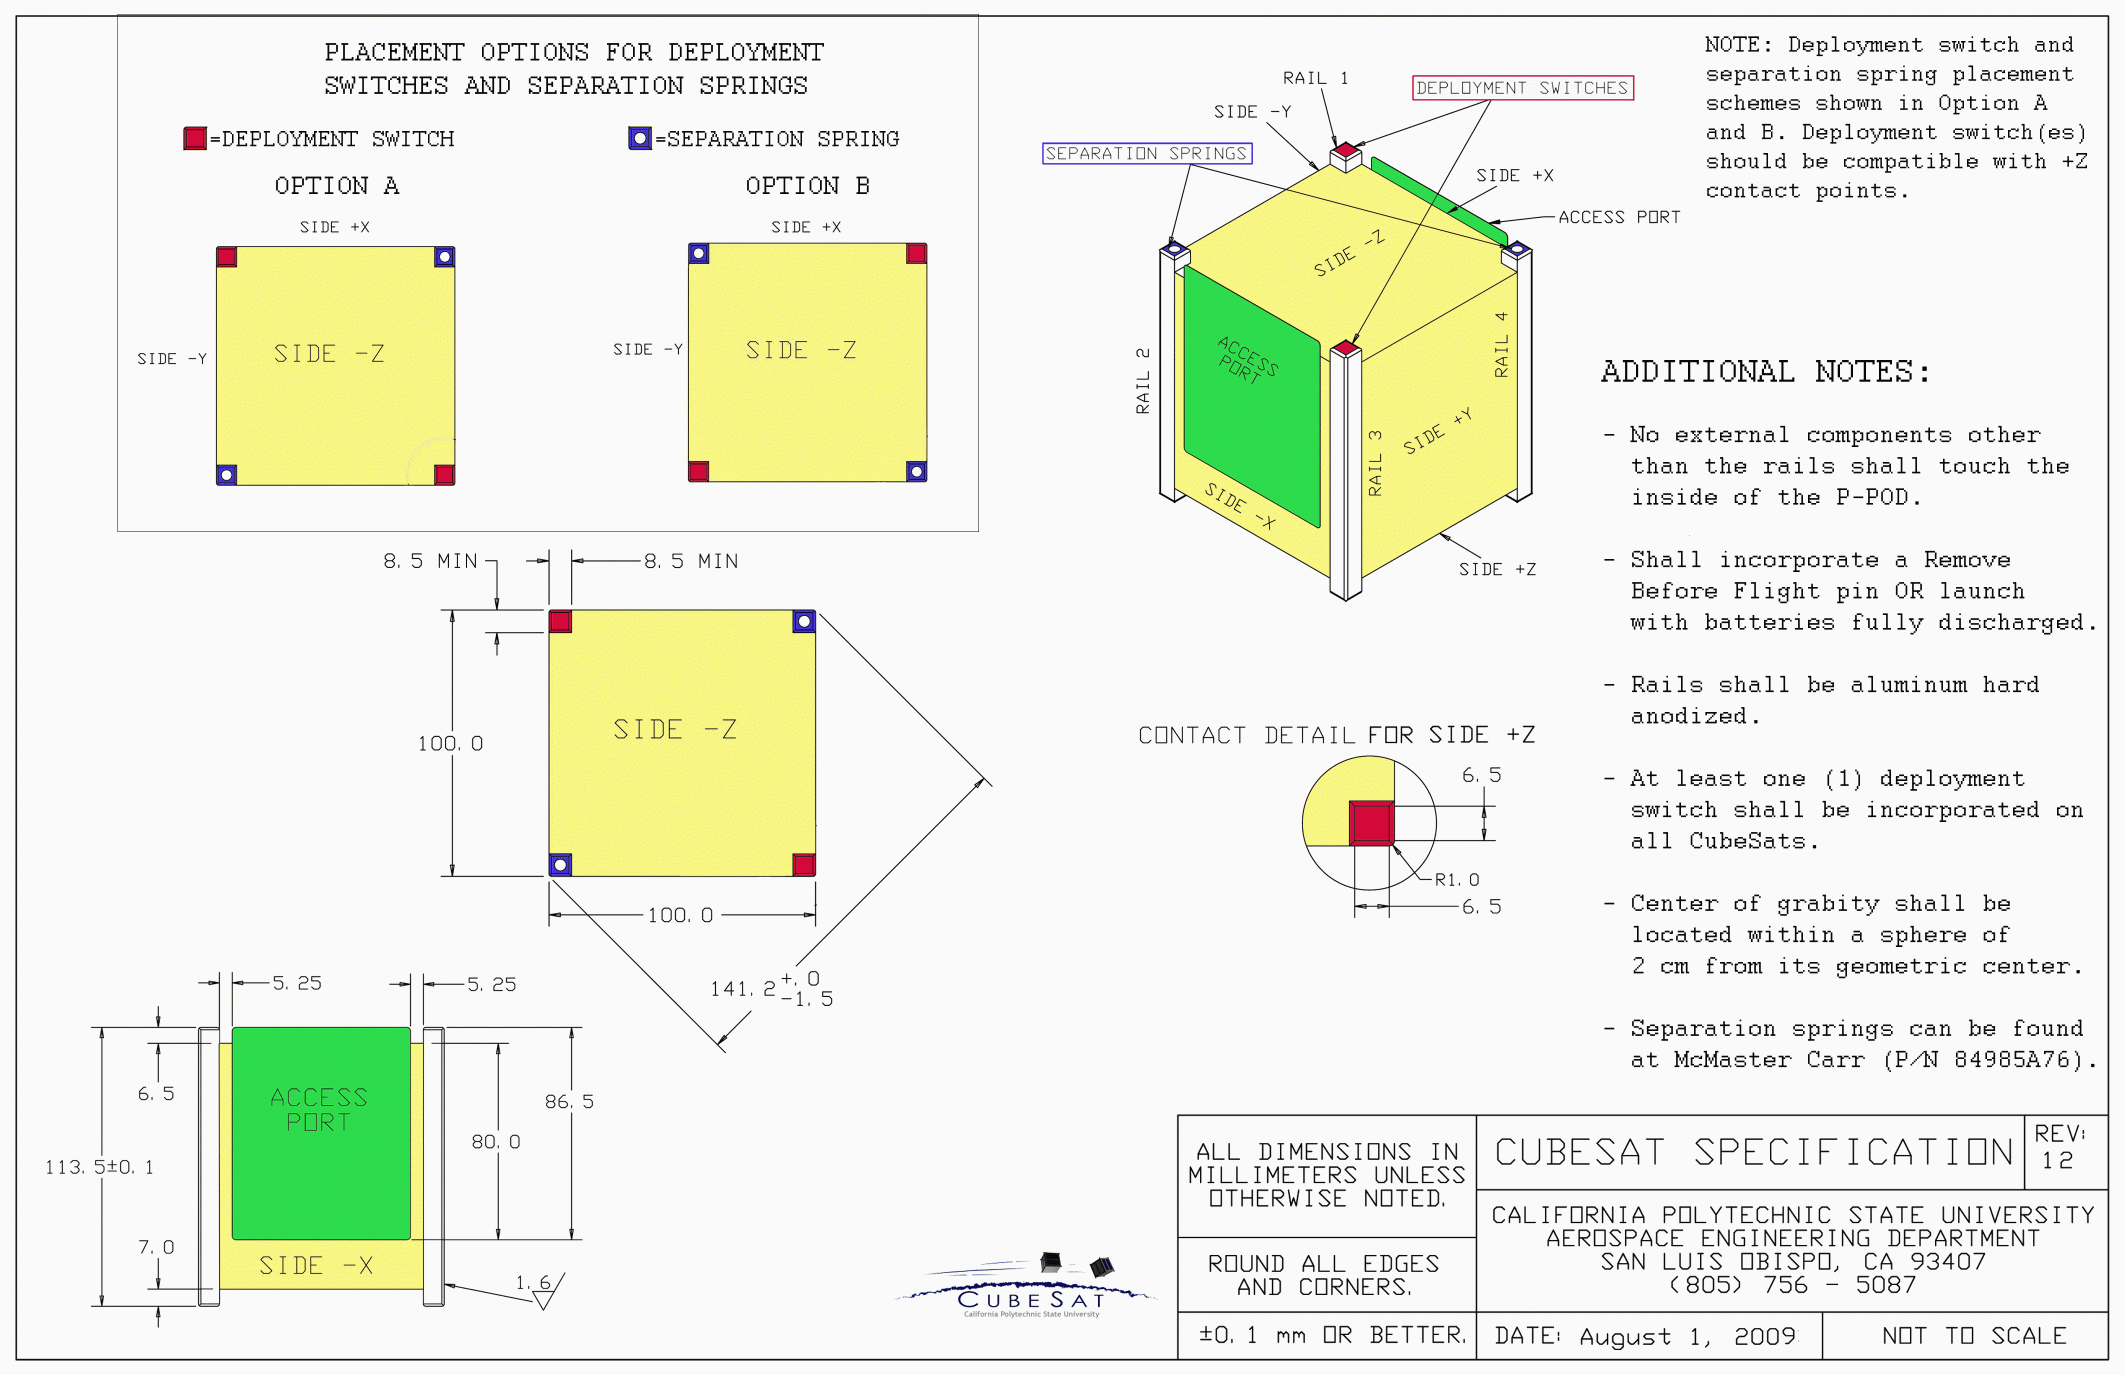
\includegraphics[scale=0.6]{./sections/SatelliteDesign/images/CubeSatDesign}
%\centering
%\caption{Dimensions of a 1U CubeSat}
%\cite{cubesatdimensions}
%\end{figure}

\subsubsection{Thermal protection}
\paragraph{}The thermal protection system consists of various insulating materials that aim to protect the CubeSat from potential thermal shocks. The satellite must remain within an optimal range of temperature, despite of the variation of the external temperature, in order to work properly. Operating in space, the CubeSat is vulnerable to suffer extreme temperatures, both below zero and above zero, and thermal protection must guarantee that all subsystems are protected. Furthermore, the thermal protection system should also dissipate the heat produced by the other systems.

\paragraph{} Currently, the most used element as thermal protection in the aerospace industry is the multilayer insulation (MLI), a set of multiple thin insulation layers. The MLI fulfills all the requirements that were previously stated and its main objective is to reduce the heat generated by radiation since the heat generated by convection or conduction does not have such a high impact on the on-board systems.

\paragraph{} 
After a market study, \textit{Dunmore Aerospace} company has been chosen to provide us its MLI product. Specially, the product is the \textbf{Dunmore Aerospace Satkit} and it is made for small satellites for LEO and it will provide the CubeSat with the protection required during operation

\subsubsection{Study of the commercial available options and options chosen}
\paragraph{}A broad marked study is needed since all the options have to be considered. For this reason, and with the aim to show all the information and features of each system that has been considered in this section, the table \ref{structureoptions} is presented below.


\begin{longtable}{| l | c | c | }
\hline
\rowcolor[gray]{0.80}	\textbf{Brand and model} &  \textbf{Features}     & \textbf{Total price (\euro)}   \\
\hline
\endfirsthead

\rowcolor[gray]{0.85} \textbf{Structure} &  &  \\
	   ~ISIS 3U structure & \makecell{Low mass (304.3g) \\ Highly compatible \\ High temperature range} & 3900 \\
	   \hline
	   ~Gomspace GOMX-Platform & \makecell{High mass (1500g) \\ Comes fully equipped (basic systems) \\ High temperature range} & 11000 \\
	   \hline
\rowcolor[gray]{0.85} \textbf{Thermal protection} &  &  \\
	   ~Dunmore Aerospace Satkit & \makecell{Lightweight \\ Durability \\ Made for small satellites}& \textbf{TO REQUEST!} \\
	   \hline
	   ~Dupont Kapton Aircraft Thermal & \makecell{Lightweight \\ Durability \\ Non-flammable} & \textbf{TO REQUEST!} \\
	\hline

\caption{Options studied for the structure and thermal protection}
\label{structureoptions}
\end{longtable}

\paragraph{}Finally, the options chosen are presented in the table \ref{structurefinal}.

\begin{longtable}{| l | r | r | r | }
\hline
\rowcolor[gray]{0.80}	\textbf{System} &  \textbf{Brand and model}     & \textbf{Price per unit (\euro)} & \textbf{N. of units}  \\
\hline
\endfirsthead

	   ~3U Structure & ISIS & 3900 & 1 \\
	   \hline
	   ~Thermal Protection & Dunmore Satkit & TO REQUEST & 1\\
	\hline

\caption{Options chosen for the structure and thermal protection}
\label{structurefinal}
\end{longtable}
